Der Wien'sche Geschwindigkeitsfilter ist eine Möglichkeit, einen Elektronenstrahl nach seiner Geschwindigkeit zu filtern, das heißt, nur Elektronen mit einer gewissen Geschwindigkeit passieren zu lassen.

\subsection{Aufbau}


Grundbaustein bildet eine Ablenkeinheit mit einem Kondensator, wie sie in der Braun'schen Röhre (Siehe: \referenz{sec:BraunscheRoehre}) verwendet wird. Allerdings wird nun ein homogenes Magnetfeld so über den Kondensator gelegt, dass die Feldlinien dieses Feldes senkrecht auf der Elektronenrichtung \emph{und} den Feldlinien des elektrischen Feldes stehen.

Abbildung \ref{fig:Wien}\endnote{„Wienscher Geschwindigkeitsfilter“ von Till Blaha - Eigenes Werk. Lizenziert unter Gemeinfrei} zeigt den schematischen Aufbau und die grobe Funktionsweise für einen Versuch mit Elektronen.

\begin{figure}[h!]
	\centering
	\vspace*{-10pt}
	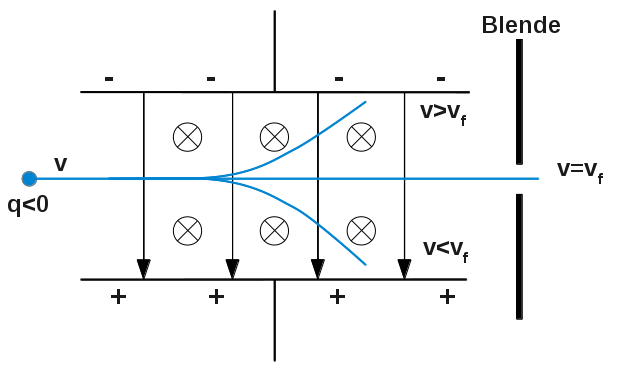
\includegraphics[width=0.8\textwidth]{WienscherFilter}
	\caption{Der Geschwindigkeitsfilter nach Wien. Die Pfeile charakterisieren die Richtung des elektrischen Feldes, die Kreuze zeigen an, dass die Richtung des Magnetfeldes in die Blattebene verläuft.}
	\label{fig:Wien}
\end{figure}

\begin{Anmerkung}
	Die magnetischen Feldlinien sind nicht direkt zeichenbar, da sie \glqq in die Papierebene\grqq{} gehen. Es wird $\odot$ verwendet, um Anzuzeigen, dass der Pfeil aus der Ebene hinaus verläuft und $\otimes$ um Anzuzeigen, dass der Pfeil in die Ebene hinein verläuft.
	
	Eselsbrücke: Wenn man mit einem Bogen einen Pfeil verschießt, sie man das Kreuz der Federn; im letzten Moment, bevor man von einem getroffen wird, sieht man den Punkt der Pfeilspitze.
\end{Anmerkung}



\subsection{Funktionsweise}

Das Magnetfeld und der Kondensator werden so gepolt, dass die, gemäß linker Handregel resultierende, Lorentzkraft $F_{Lr}$ der Coulombkraft $F_{el}$ entgegenwirkt. Da die Lorentzkraft abhängig von der Geschwindigkeit des Elektrons ist und die elektrische Kraft nicht, gibt es eine Geschwindigkeit $v_f$, bei der sich die beiden Kräfte die Waage halten. Dies ist die Geschwindigkeit, die vom Filter durchgelassen wird:

\begin{align}
\begin{split}
	F_{Lr} &= F_{el} \\
	q_e \cdot B \cdot v_f &= q_e \cdot E \\
	v_f &= \frac{E}{B}
\end{split}
\end{align}

\noindent \emph{Man nehme Notiz von dieser simplen und unglaublich schönen Beziehung!}

Eine Einheitenrechnung folgt und zeigt, dass die Einheiten aufgehen:

\begin{align}
\begin{split}
	v_f &= \frac{E}{B} \\
	\frac{m}{s} &= \frac{N}{C} \cdot \frac{1}{T} \\
	\frac{m}{s} &= \frac{kg \cdot m}{s^2 \cdot As} \cdot \frac{As^2}{kg} \\
	\frac{m}{s} &= \frac{m}{s}
\end{split}
\end{align}
